In this section we will explore the data set from HOME that is to be analysed in this project.
The data set consists of information regarding house sales in the period from 2004 to 2016.
It has 131.920 observations where the price as well as some additional information on the house in question has been recorded.
Following a preliminary examination of the data set we have chosen to focus on apartments in the four largest danish cities. 
These being Copenhagen, Aarhus, Odense and Aalborg.
For the variables we have chosen to focus on
\begin{enumerate}
    \item Property Condition (Bad, Okay, Good)
    \item Size in $m^2$
    \item Year of sale
    \item Days until the property was sold
    \item Construction year
    \item Number of bedrooms
    \item Balcony or not
    \item Renovation or not
\end{enumerate}
Restricting to the cities in question results in a reduction of the number of observations.
The number of observations after the reduction is 8.497.
How the observations are distributed between the cities can be seen on figure \ref{fig:distributions_between_cities}.
\begin{figure}[H]
    \centering
    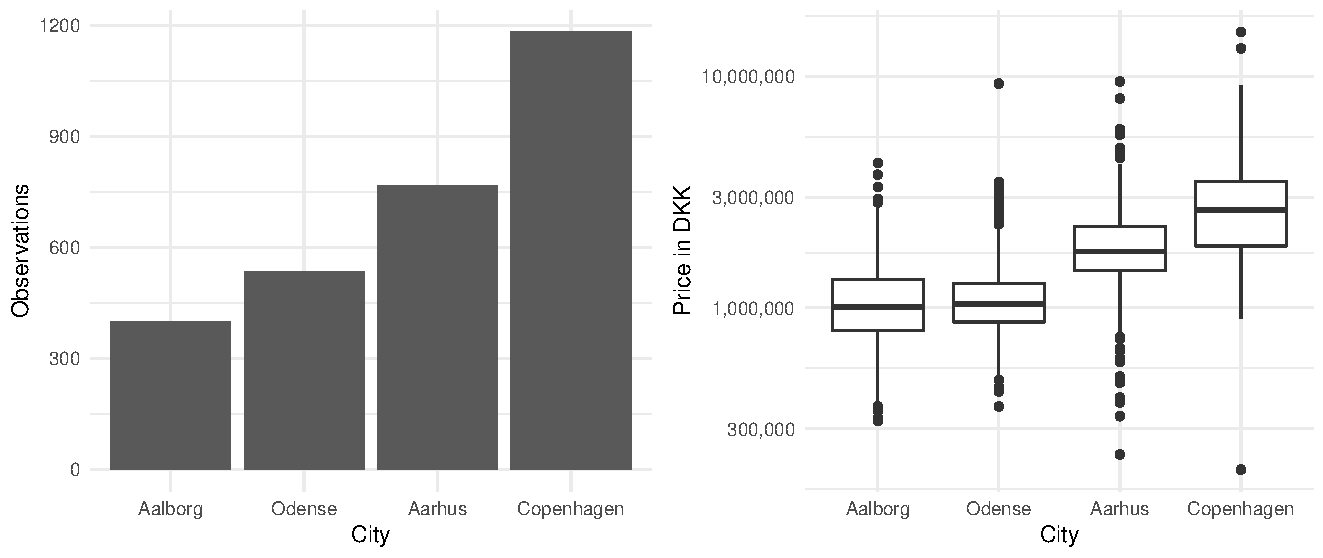
\includegraphics[width=\textwidth]{figures/Data_introduction/distribution_between_cities.pdf}
    \caption{Distribution of observations and box plot of price between the cities.}
    \label{fig:distributions_between_cities}
\end{figure}
Here it is seen that most observations are from Copenhagen, which is to be expected as there are more property than in the other 3 cities.
We can also note the differences in the average price between the cities indicating that, all else equal just knowing the city in which the apartment is located tells something about its price.